\section{KNN}
This chapter will give information on the classification method called KNN (K nearest neighbour).\\
Shortly put in \citep{meaningfulNN} the NN is "given a collection of data point and query points in an m-dimentional metric space, find the data point that is closets to the query point".\\
If going into more detail the above sentence will mean that the NN classification will need a dataset often refereed to as the training data, the data in the training set has to be notated so that the program that make the classification knows what is in the dataset. When one has the training data set with notation they need some value to describe what sound it is  because even though notated they can still be different in how they sound e.g two people might say a sound different from another, for this one can make use of different features to describe these differences. Then the training data can be see as being scattered out on a field based on what value they have from the feature. Now when there comes a new input, the input can be given a value from the features. Then based the placement on the field the new data get it can look at the sounds that are close to it, the input sound neighbour. Then with KNN the K will then be how many neighbours that has to be look at before determining what the new input is, then the most represented sound will be chosen as what the input sound is. Another way that one can choose the nearest neighbour is by look at all the neighbour inside some distance (euclidean distance)\citep{NNHD}.

\begin{figure}[h]
	\begin{center}
		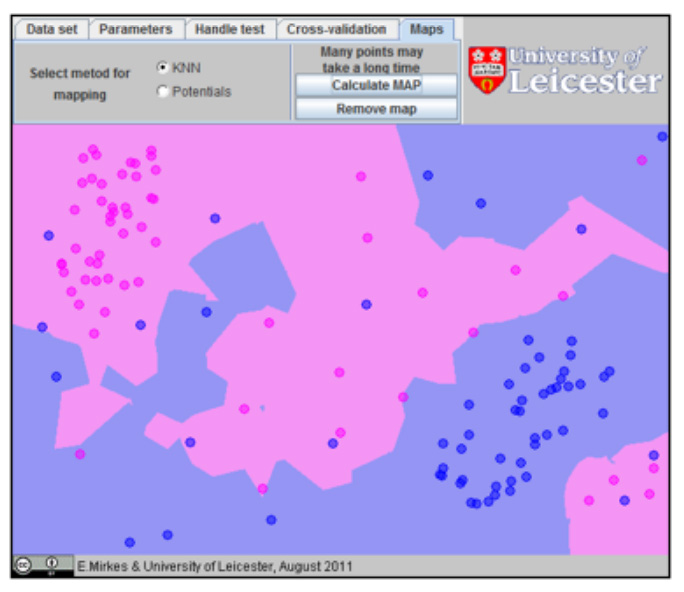
\includegraphics[scale = 0.5]{fig/KNNfig.jpg}
		\caption{KNN field here one can see how the knn will divide the space up with to different classes \citep{introKNN}}
		\label{KNN fig}
	\end{center}
\end{figure}
